\begin{figure}[h]
    \centering
    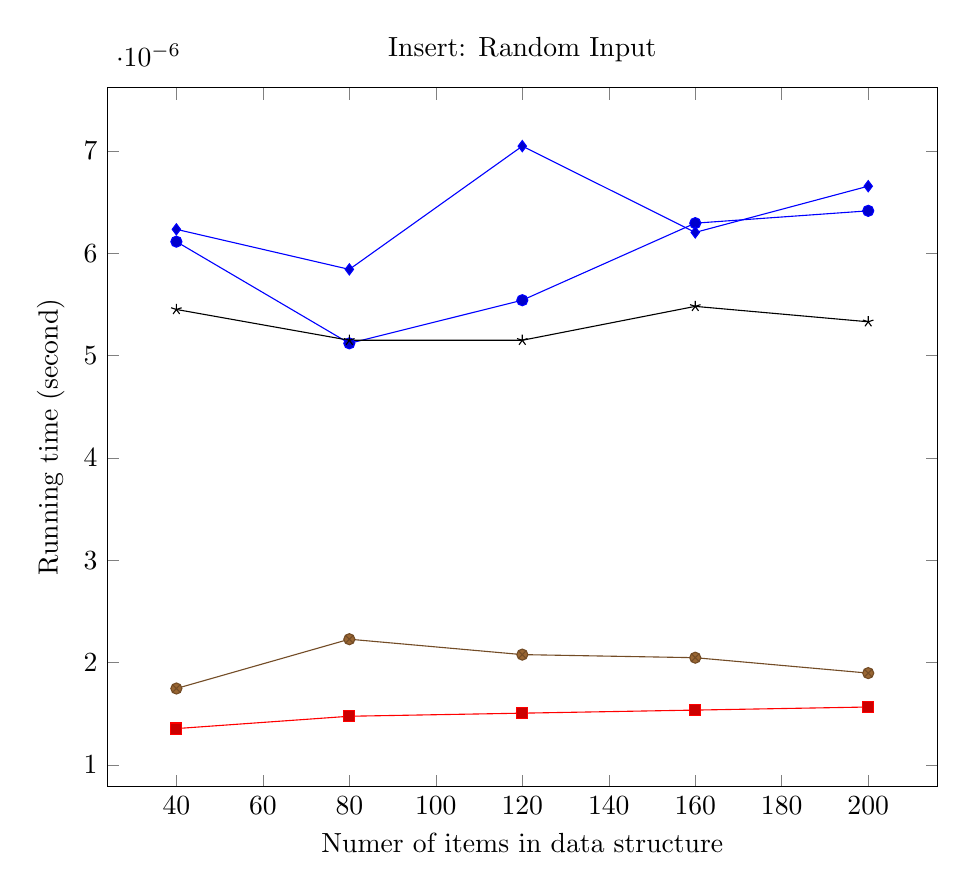
\begin{tikzpicture}
        \begin{axis}[
            xlabel={Numer of items in data structure},
            ylabel={Running time (second)},
            title={Insert: Random Input},
            width=\textwidth
        ]
		\addplot coordinates {
			(40, 6.113859336309701e-06)
			(80, 5.1199807245438935e-06)
			(120, 5.541626196148286e-06)
			(160, 6.2945645378675865e-06)
			(200, 6.415034672713204e-06)
		};
		\addplot coordinates {
			(40, 1.355289015236849e-06)
			(80, 1.4757591500824673e-06)
			(120, 1.5058766834386005e-06)
			(160, 1.5359942175052766e-06)
			(200, 1.5661117508614098e-06)
		};
		\addplot coordinates {
			(40, 1.7468169531298372e-06)
			(80, 2.2286974921570392e-06)
			(120, 2.0781098236000163e-06)
			(160, 2.0479922898886117e-06)
			(200, 1.89740462168686e-06)
		};
		\addplot coordinates {
			(40, 5.4512735950140724e-06)
			(80, 5.150098258255298e-06)
			(120, 5.150098258255298e-06)
			(160, 5.481391128725477e-06)
			(200, 5.330803460523726e-06)
		};
		\addplot coordinates {
			(40, 6.234329470800048e-06)
			(80, 5.842801532907061e-06)
			(120, 7.047502879942158e-06)
			(160, 6.204211937088644e-06)
			(200, 6.65597494204917e-06)
		};
        \legend{}
        \end{axis}
    \end{tikzpicture}
    \caption{Average of 0 operations, benchmarked every 0, starting at 0.}
\end{figure}